\documentclass[letterpaper,twocolumn,10pt]{article}
\usepackage{epsfig,xspace,url}
\usepackage{authblk}
\usepackage{graphicx}
\graphicspath{ {images/} }

\title{CS 6480: Lab Assignment 1\\
Mininet - Software Defined Networking}
\author{Damodar Sahasrabudhe}
\affil{School of Computing, University of Utah}

\begin{document}

\maketitle

\section{Tasks Completed}
\begin{itemize}
\item Installed SDN VM.
\item Went through papers the "Mininet Walkthrough" and the "Introduction to Mininet" and tried commands and other configuration on VM
\item Traced network traffic using Wireshark.
\item Went through OpenFlow implementations and tutorial papers.
\item Partially understood how POX is working. 
\item Completed controller setup using POX for static - hardcoded IPs and ports. Inserted table entries for ARP and for HTTP. Hosts are able to ping each other. See Figure 1.
\item Set one host as http server and send request from another node. Request and response were successful. See Figure 2.


\begin{figure}[h]
\caption{Entries for ARP and HTTP}
\centering
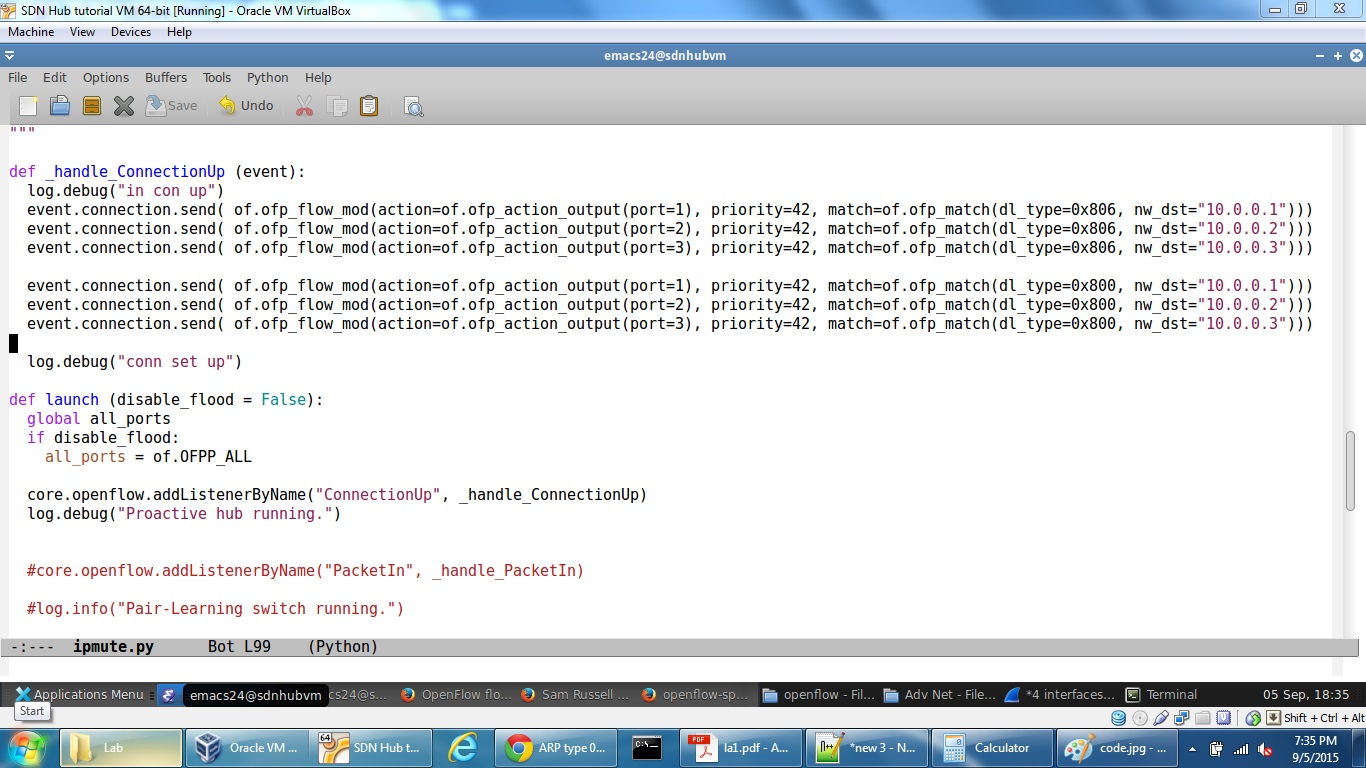
\includegraphics[width=\textwidth]{code}
\end{figure}

\begin{figure}[h]
\caption{Demo of ping and http request}
\centering
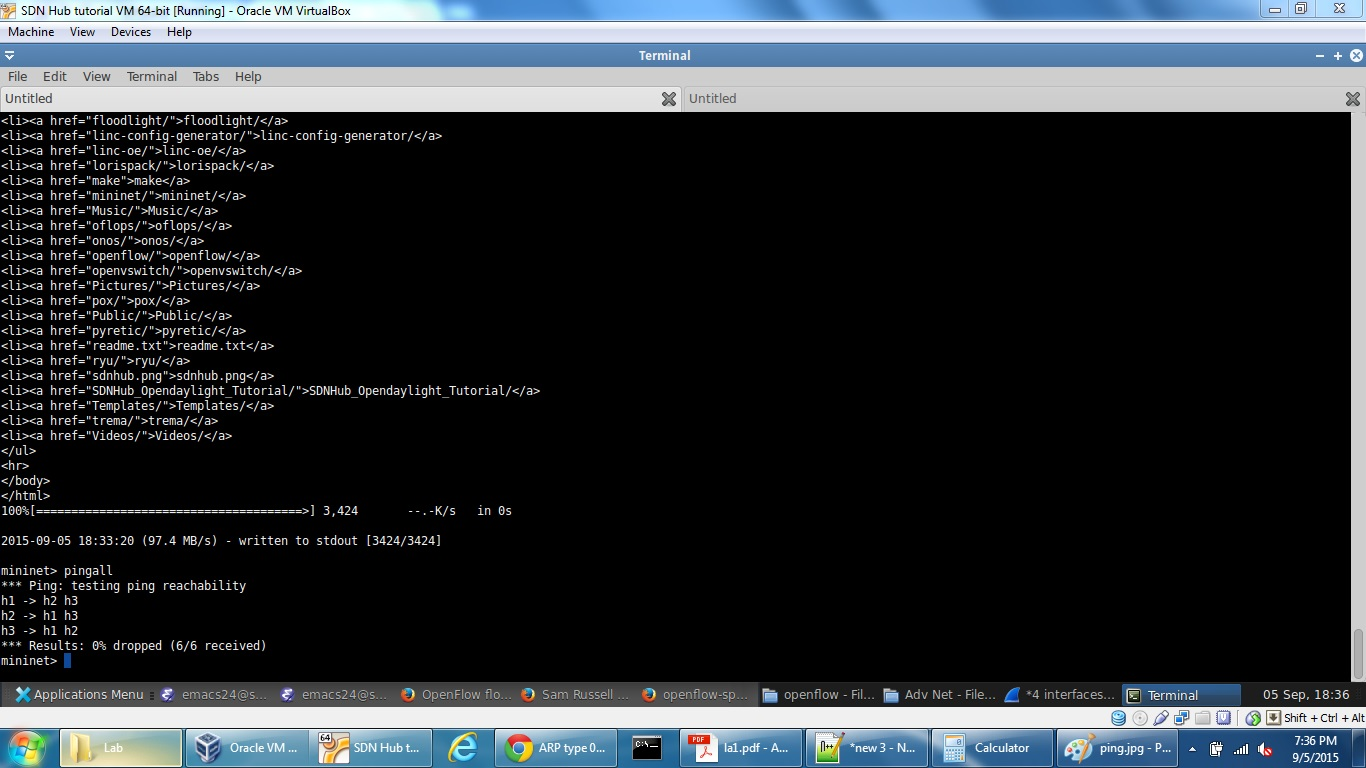
\includegraphics[width=\textwidth]{ping}
\end{figure}


\section{Hurdle}
During random mutation of IP address, DNS will respond to external node with a fake IP. So external node will send requests destined for fake IP. Even if switch routes those requests to real web server, destination IP in the packet will not match with IP of web server. So web server will reject those packets. In this case, action in switch should change IP in packet and then route. (Is it right? if yes how? In case of yes, when response is sent back to external node, source ip should be changed back to original fake ip)


\section{Tasks Planned Next week}
\item Implement DNS look up.
\item Build action to exchange packets using "fake" ip.
\item Action should change destination ip to real ip while routing request to web server and should change source ip to fake ip while sending response to node.

\end{itemize}

{
  %\footnotesize 
  \small 
  \bibliographystyle{acm}
  \bibliography{biblio}
}
\end{document}



